\documentclass[11pt,a4paper]{article}

% ------------------------------------------------------------------
% Standalone, self-contained working document. NOT wired into the main
% thesis.tex build and NOT meant to be dropped into 03_Content/4_Results.tex
% as-is. Covers the SECOND-generation ("v2") corpus and shared space --
% see thesis/corpus/ANALYSIS_OVERVIEW.md's "Extraction pipeline v2" section
% and thesis/03_Content/3_Methods.tex's "Revising the Extraction Pipeline"
% for why v2 exists at all. The predecessor v1 document,
% thesis/04_Appendix/Geometric_Analysis_Draft/geometric_analysis_report.tex,
% covers the frozen, still-on-disk v1 run and is kept for comparison.
%
% This is a full rewrite of the first v2 report (which covered run
% 20260909-224215). That run's emergent-entities layer turned out to be
% badly under-powered -- 21 entities total, mostly single-mention noise,
% zero shared across all three corpora -- traced to a real bug (entity
% extraction only looked inside already-kept expressions) rather than a
% genuine property of the corpus. This report covers the corrected run
% (20260910-010254): entities are now also pulled from a broader,
% previously-unused extraction field, filtered for named-entity shape,
% and cross-checked against this corpus's own cited-author list. Where
% useful, this document shows the before/after directly rather than
% hiding the correction.
%
% Includes a labelled "Possible interpretations" section and a plain-
% language summary, at the researcher's explicit request -- kept visibly,
% structurally separate from the descriptive-fact sections and flagged
% throughout as provisional readings for the researcher to argue with,
% not the thesis's settled Results-chapter conclusions.
% Compile directly: pdflatex geometric_analysis_report_v2.tex
% ------------------------------------------------------------------

\usepackage[a4paper,margin=2.7cm]{geometry}
\usepackage[utf8]{inputenc}
\usepackage[T1]{fontenc}
\usepackage{graphicx}
\usepackage{booktabs}
\usepackage{longtable}
\usepackage{array}
\usepackage{xcolor}
\usepackage{enumitem}
\usepackage{caption}
\usepackage{parskip}
\usepackage[colorlinks=true,linkcolor=blue!50!black,citecolor=blue!50!black,urlcolor=blue!50!black]{hyperref}
\usepackage{titlesec}
\usepackage{tabularx}

\definecolor{noteback}{RGB}{240,240,248}
\definecolor{noteline}{RGB}{120,120,180}
\newenvironment{plainbox}[1][Note]
  {\par\vspace{6pt}\noindent{\color{noteline}\rule{\linewidth}{0.6pt}}\par\vspace{3pt}
   \noindent\small\textbf{#1.}\ \ignorespaces}
  {\par\vspace{3pt}\noindent{\color{noteline}\rule{\linewidth}{0.6pt}}\vspace{6pt}\par}

\definecolor{interpline}{RGB}{180,140,60}
\newenvironment{interpbox}[1][Possible interpretation]
  {\par\vspace{6pt}\noindent{\color{interpline}\rule{\linewidth}{0.8pt}}\par\vspace{3pt}
   \noindent\small\textcolor{interpline}{\textbf{#1.}}\ \ignorespaces}
  {\par\vspace{3pt}\noindent{\color{interpline}\rule{\linewidth}{0.8pt}}\vspace{6pt}\par}

\definecolor{fixline}{RGB}{60,140,90}
\newenvironment{fixbox}[1][What was fixed]
  {\par\vspace{6pt}\noindent{\color{fixline}\rule{\linewidth}{0.8pt}}\par\vspace{3pt}
   \noindent\small\textcolor{fixline}{\textbf{#1.}}\ \ignorespaces}
  {\par\vspace{3pt}\noindent{\color{fixline}\rule{\linewidth}{0.8pt}}\vspace{6pt}\par}

\newcommand{\jargon}[1]{\textbf{#1}}

\title{\textbf{Mapping "Cult," Second Pass: The v2 Geometric Analysis}\\[4pt]
\large Working report -- draft base material for the Results chapter,\\
with a first attempt at interpretation}
\author{Prepared for C\'elestin Meunier's thesis project}
\date{Covers run \texttt{20260910-010254}, generated 2026-09-10}

\begin{document}
\maketitle

\begin{plainbox}[How to read this document]
This is still not a finished Results chapter. Sections~\ref{sec:stages}--\ref{sec:honesty}
report numbers, not arguments. Section~\ref{sec:interpretation} is a first,
explicitly provisional pass at what these patterns \emph{might} mean, kept
structurally separate and visually marked (a tan box) throughout so a
reader can tell at a glance which sentences are geometric fact and which
are a reading of that fact the researcher is free to revise or reject.
Green boxes mark a specific, checkable methodological correction made
during this run, with what was wrong and how it was verified fixed --
included because the correction itself is informative about how much to
trust a "count of named things" figure in general. Nowhere in this
document is geometric proximity treated as evidence that any group,
practice, or person \emph{is} or \emph{is not} "a cult."
\end{plainbox}

\tableofcontents

% ============================================================
\section{In short: what did this run find?}
\label{sec:short}
% ============================================================

\begin{itemize}[leftmargin=1.4em]
  \item \textbf{The corpus got much smaller, on purpose} (same as the
  first v2 pass): a stricter, judge-verified extraction pipeline cut
  literature from 39,236 to 5,741 expressions, trading quantity for
  verified fidelity.
  \item \textbf{The three sources still barely form separate geometric
  clusters} -- silhouette near zero, same conclusion as before.
  \item \textbf{A real bug was found and fixed in how "emergent
  entities" (named groups/leaders the corpora talk about) were counted.}
  The first v2 pass found only 21 entities, almost all mentioned exactly
  once, zero shared across all three corpora. That was not a fact about
  the corpus -- it was because entity extraction only looked inside
  expressions that survived the strict extraction filter, silently
  discarding named-entity mentions sitting in text that didn't. Fixed,
  this run finds \textbf{753} entities, including \textbf{3 mentioned by
  all three corpora at once} ("New Age," Jehovah's Witnesses in French,
  and the Order of the Solar Temple) and \textbf{55 mentioned only in
  interviews} (up from 0). Full story in Section~\ref{sec:entities}.
  \item \textbf{Named things still sit at the edge of their own corpus's
  "typical" region; generic statements sit near the centre} -- same
  pattern as before, unaffected by the entity fix (it concerns ordinary
  expressions, not the entity layer).
  \item \textbf{The "Sept?" data-quality finding from the first pass
  still stands} -- one interview response, almost certainly a mishearing
  of \emph{secte} as \emph{sept}, passing every automated check. Still
  1 point out of the space; still not large enough to change any result.
\end{itemize}

% ============================================================
\section{Where the project stands}
\label{sec:stages}
% ============================================================

\subsection{Why a second pass at all}
A 100-item manual fidelity review of the first extraction pipeline
(2026-09-08) found it systematically over-inclusive: paraphrased or
mistranslated expressions, document headings and bibliography citations
extracted as though they were claims, occasional interviewer questions
mislabelled as participant statements. The pipeline (\jargon{v2}) was
rebuilt around a strict verbatim-span rule plus a second, independently-
prompted model that judges every retained candidate the way a human
reviewer would ("model-judged," never a substitute for human review).
v1's own archives and every retained run stay frozen on disk, untouched.

\subsection{Stage 1--2 -- Same three corpora, far fewer expressions}
Same underlying documents as v1 (57 scholarly works, 2 MIVILUDES
documents, 26 interview transcripts); far stricter extraction:

\begin{table}[h!]
\centering
\begin{tabular}{lrrr}
\toprule
Corpus & v1 expressions & v2 expressions & Change \\
\midrule
literature & 39{,}236 & 5{,}741 & $-85.4\%$ \\
MIVILUDES & 914 & 108 & $-88.2\%$ \\
interviews & 230 & 64 & $-72.2\%$ \\
\bottomrule
\end{tabular}
\end{table}

\subsection{Stage 3--4 -- Reference vocabularies unchanged; emergent entities, twice}
The three reference vocabularies (concept backbone, structural concepts,
ConceptNet-generalised concepts) are unchanged from v1, reused as-is.
Emergent entities were built \emph{twice} this session -- the first
attempt undercounted badly; see Section~\ref{sec:entities} for the full
story and the fix.

\subsection{Stage 5 -- One shared geometric space, rebuilt}
Same pooling procedure as v1: embed everything with the same model,
standardize, PCA down to the smallest dimensionality keeping 95\% of the
variance. With the corrected, much larger emergent-entities layer, this
run's space holds \textbf{11,378} points, compressed to \textbf{393}
dimensions (95.0\% variance kept) -- up from the first v2 pass's 10,646
points/389 dimensions, entirely due to the extra 732 entity points now
correctly included.

\subsection{Stage 6 -- The interview "first impression" layer: ported, not redone}
Unchanged from the first v2 pass: the 25 manually-verified interview
opening-prompt exemplars are re-projected through this run's transform
rather than re-selected -- the embedding of a quote is a property of its
own words, not of which build happened to be running.

\subsection{Stage 7 -- The equal-$n$ correction still applies, at a smaller scale}
Unchanged finding from the first v2 pass: literature is still
\textbf{97.09\%} of expression points (the emergent-entities fix does
not touch expression counts), so the same equal-$n$/equal-size
corrections are still necessary and still used, drawing 64 points per
source (down from v1's 204).

\subsection{Stage 8 -- Two toolkit runs, one throwaway}
The reusable 10-module analysis toolkit was run against this shared
space twice this session: once against the (bugged) 21-entity space,
and again -- covered by this document -- after the fix, against the
corrected 753-entity space (run \texttt{20260910-010254}). The first
run's own report is not being kept as a separate document; this report
supersedes it. A fresh spot-check sample (Section~\ref{sec:spotcheck})
was drawn from the retained v2 extraction output before either toolkit
run and is unaffected by the entity-layer fix (it concerns expression
extraction, not entities).

% ============================================================
\section{Key ideas, explained in plain language}
\label{sec:jargon}
% ============================================================

Unchanged from earlier documents -- included again so this one is
self-contained. Skip if already familiar.

\subsection{Embeddings, distance, and similarity}
An \jargon{embedding} converts a piece of text into a long list of
numbers (a \jargon{vector}, 1,024 numbers here) such that similar
meanings end up as nearby vectors. \jargon{Euclidean distance} is
ordinary straight-line distance in that many-dimensional space (smaller
= more similar). \jargon{Cosine similarity} instead measures whether two
vectors point in the same \emph{direction} from the origin, ignoring
length ($-1$ opposite, $1$ identical direction, $0$ unrelated). Both are
always reported side by side.

\subsection{Centroid, standardization, and PCA}
A \jargon{centroid} is a group of points' average position -- literature's
"average position," MIVILUDES's, and so on. Every dimension was
\jargon{standardized} before pooling so no source dominates purely
because its raw numbers are larger. \jargon{PCA} then compresses the
1,024-number description of each point down to the smallest number of
dimensions keeping 95\% of the original variation -- 393 dimensions this
run. Every distance/similarity number below is computed in this
393-dimensional space.

\subsection{UMAP, k-NN composition, and silhouette}
\jargon{UMAP} produces an approximate, readable 2-D layout purely for
visualisation -- not itself evidence. A point's \jargon{k nearest
neighbours} are the $k$ closest other points ($k{=}10,20$ here);
averaging their source-composition over many points asks how much
different sources overlap versus occupy separate regions. \jargon{Silhouette}
scores (roughly $-1$ to $1$) how well a proposed grouping matches the
data's actual geometric clustering; near 0 means the groups don't
correspond to distinct clusters.

\subsection{Bootstrap confidence intervals; equal-size/equal-$n$ comparisons}
"Mean, 95\% CI [low, high]" comes from \jargon{bootstrap resampling}:
repeating a measurement 100 times on randomly resampled subsets. The
three expression sources (5,741/108/64 this run) and the three reference
vocabularies (3,000/1,500/195) are wildly different sizes; an
\jargon{equal-size-controlled} comparison down-samples every set to the
smallest before comparing, controlling for pool-size bias specifically
-- not evidence the sets are otherwise interchangeable.

\subsection{Typicality and "borderline" points}
A point's \jargon{typicality} is simply how close it sits to its own
group's centroid -- close = "typical," far = "atypical," a purely
geometric fact about this space under this model, not a claim about
cognitive prototypicality or real-world category membership. A
\jargon{borderline} point between groups $A$/$B$ is one whose distances
to each centroid are nearly equal.

\subsection{"Point role," "source dataset," and provenance categories}
\jargon{source\_dataset}: which of the eight underlying datasets a point
came from. \jargon{point\_role}: expression / reference / emergent.
Every emergent entity also carries a \jargon{provenance category} --
\texttt{literature\_only}, \texttt{miviludes\_only},
\texttt{interviews\_only}, \texttt{shared\_2\_corpora}, or
\texttt{shared\_all\_3} -- describing only which corpora mention it, not
any normative claim about the entity itself.

% ============================================================
\section{The datasets pooled into the shared space}
% ============================================================

\begin{table}[h!]
\centering
\small
\begin{tabularx}{\textwidth}{@{}l r l X@{}}
\toprule
\textbf{Source} & \textbf{Points} & \textbf{Role} & \textbf{What it is} \\
\midrule
literature & 5{,}741 & expression & Strict-verbatim extraction, 57 scholarly works \\
miviludes & 108 & expression & Strict-verbatim extraction, 2 MIVILUDES documents \\
interviews & 64 & expression & Strict-verbatim extraction, 26 interview transcripts \\
miviludes\_criteria & 17 & expression & MIVILUDES's 17 official sectarian-drift criteria (unchanged) \\
concept\_backbone & 3{,}000 & reference & Topic-neutral WordNet-derived concepts (unchanged) \\
structural\_concepts & 1{,}500 & reference & Corpus-mined structural/relational vocabulary (unchanged) \\
conceptnet\_concepts & 195 & reference & Hand-reviewed ConceptNet generalisation (unchanged) \\
emergent\_entities & \textbf{753} & emergent & Named entities, corrected this run -- see Section~\ref{sec:entities} \\
\bottomrule
\end{tabularx}
\caption{The eight sources pooled into the 11{,}378-point, 393-dimensional v2 shared space.}
\end{table}

A ninth, separate layer -- 25 ported interview prototypes -- sits in the
same coordinate system but is not part of this count or the PCA fit.

% ============================================================
\section{Spot-check: is this run's data trustworthy?}
\label{sec:spotcheck}
% ============================================================

Carried over unchanged from the first v2 pass -- this concerns expression
extraction quality, not the entity-layer fix below, so it does not need
repeating. A fresh random sample was drawn from each corpus's final,
judge-accepted output (100 literature, 40 MIVILUDES, 30 interview
expressions; seed 42; full methodology in
\texttt{processed/audits/v2\_spotcheck\_20260909.md}). Automated checks
found 0 verbatim/faithfulness failures across 170 sampled rows. An
independent read found expressions correctly attributed and sensibly
tagged throughout, with one genuine, small finding:

\begin{plainbox}[One genuine finding: "Sept?"]
Interview \texttt{b3-aug23-1213} (participant, age 97), asked in French
"\emph{Quand je te dis le mot secte à quoi tu penses?}" ("When I say the
word `secte' [cult], what do you think of?"), answered \textbf{"Sept?"}
("seven?") -- almost certainly a mishearing of \emph{secte} as
\emph{sept}, not a substantive response. The judge model scored it
faithful/self-contained/cult-relevant/atomic, correctly noting it is a
genuine transcript quote -- true, but the string carries no propositional
content about cults. Scale: 1 of 11,378 points (0.01\%). Left in place,
unmodified, as an explicit, logged limitation.
\end{plainbox}

% ============================================================
\section{Emergent entities: found, broken, and fixed}
\label{sec:entities}
% ============================================================

This section gets its own, expanded treatment because the correction
made here is the main methodological story of this run, and because
understanding \emph{why} it was wrong is useful for judging how much to
trust the corrected number.

\subsection{What went wrong}

The first v2 toolkit run found only \textbf{21} emergent entities --
20 literature-only, 1 miviludes-only, 0 interviews-only, 0 shared by any
two or three corpora -- almost all mentioned exactly once. This looked
implausible on inspection: several of the 21 were not really named
entities at all ("leadership," "desert," "post-Soviet remaking of
identities" -- generic phrases, not named things), and the corpus was
known independently (Section~\ref{sec:spotcheck}, the miviludes/interviews
domain\_terms counts below) to discuss dozens of well-known groups by
name.

\begin{fixbox}[Root cause]
Entities were being extracted only from \texttt{entity\_anchors}, a
field the extraction model fills in \emph{only for expressions that
already survived} the strict verbatim+judge screening
(\texttt{extraction\_v2\_schema.py}: "named groups, leaders, movements
mentioned \textbf{in the span}"). Since that screening now keeps only
14--28\% of what v1 kept per corpus, roughly 75--85\% of named-entity
mentions sitting inside now-rejected spans were silently discarded --
even when the surrounding text discussing that entity was perfectly
legitimate, just not judged a standalone \emph{claim} worth keeping.

The fix uses a second field the extraction model already produces but
that was never wired into the shared space: \texttt{domain\_terms} --
"cult-related concepts or named groups that appear in the text, even if
no expression around them is worth keeping." Checked directly: literature
alone has 52{,}179 unique \texttt{domain\_terms} (100{,}031 mentions)
against the 20 \texttt{entity\_anchors}-only entities previously used.
\end{fixbox}

\subsection{Getting to a clean list: two more problems, found and fixed}

\texttt{domain\_terms} is a much broader net than \texttt{entity\_anchors}
-- it mixes genuine named entities ("Scientology," "Heaven's Gate") with
generic domain vocabulary ("cults," "brainwashing," "mind control") that
already has its own home in the structural\_concepts/concept\_backbone
reference vocabularies. Two further checks against real data were needed
before the result was trustworthy:

\begin{fixbox}[Casing filter, and a bug in it]
Checked directly: \texttt{domain\_terms} terms in their original,
un-lowercased casing split cleanly -- capitalized terms are almost
entirely genuine named entities (ISKCON, Branch Davidians, UNADFI);
all-lowercase terms are almost entirely generic vocabulary
(secularization, deprogramming, mind control). A simple "not all
lowercase" filter was applied to \emph{both} \texttt{domain\_terms} and
(newly) \texttt{entity\_anchors} -- the latter had never had any type
filtering at all, which is exactly why v1's top-mentioned "entity" was
"charismatic leader" (3,417 mentions, 2nd highest overall) and why v2's
first pass still let "leadership"/"desert" through. One bug found in the
filter itself: Python's \texttt{str.islower()} is \texttt{False} for a
string with \emph{no} cased characters at all, so bare years and page
numbers ("2004," "11") were passing as if capitalized. Fixed by requiring
at least one actual letter.
\end{fixbox}

\begin{fixbox}[Cited-author contamination]
Even after the casing fix, the single largest remaining source of noise
in literature was bare surnames of \emph{this corpus's own cited
authors} -- academic citations like "(Richardson 1985)" leave a bare
capitalized surname in the text, indistinguishable by casing or frequency
alone from a genuine named entity. Checked directly: "richardson" alone
had 47 mentions (more than most real cult groups); "barker" 34;
"anthony" 28. A frequency threshold cannot separate self-citation from a
genuinely important recurring entity -- both look identical (a
capitalized word mentioned often). Fixed with a targeted, data-derived
stop-list: every author surname is read directly from
\texttt{metadata/literature.csv} (the corpus's own 57-document
bibliography, 90 unique surnames) and excluded -- no hardcoded name
list, automatically correct if the corpus grows. \textbf{Not} fixed:
externally-cited classical theorists who are not themselves corpus
authors ("weber," "freud," "wallis" all still pass) -- flagged as a
known residual limitation, not silently hidden.
\end{fixbox}

\subsection{Per-corpus, not global, mention thresholds}

A single mention-count threshold applied to the cross-corpus total would
still favour literature's citation-heavy volume unfairly: a name
mentioned a handful of times there is plausibly just a citation, while
the same count in MIVILUDES/interviews' much smaller, curated text is
comparatively far more likely to be deliberate. This run uses
\textbf{per-corpus} thresholds -- literature $\geq 10$, MIVILUDES $\geq 3$,
interviews $\geq 1$ -- and an entity qualifies if it clears \emph{any
one} corpus's own threshold.

\subsection{The result}

\begin{table}[h!]
\centering
\begin{tabular}{lrr}
\toprule
Provenance category & First v2 pass (buggy) & This run (fixed) \\
\midrule
literature\_only & 20 & 603 \\
miviludes\_only & 1 & 26 \\
interviews\_only & 0 & 55 \\
shared\_2\_corpora & 0 & 66 \\
shared\_all\_3 & 0 & 3 \\
\midrule
\textbf{Total} & \textbf{21} & \textbf{753} \\
\bottomrule
\end{tabular}
\caption{Emergent-entity counts, before and after the fix.}
\end{table}

\begin{figure}[h!]
\centering

\includegraphics[width=0.7\textwidth]{figures/entity_provenance_categories.png}
\caption{Emergent entities grouped by which corpus/corpora mention them, this run.}
\end{figure}

Top entities by total mentions are now entirely genuine named
groups/movements: NRMs (685), Scientology (299), New Age (270), Heaven's
Gate (268), Unification Church (250), Jehovah's Witnesses (211), Branch
Davidians (159), Jonestown (156), Solar Temple (136), ISKCON (123),
Children of God (118), Theosophy (109), Aum Shinrikyo (103), Satanism
(95), Soka Gakkai (86) -- contrast v1's top entities, which included
"charismatic leader" (2nd highest) and bare generic nouns ("cults,"
"religion," "church," "followers").

\textbf{The 3 entities mentioned by all three corpora}: "new age" (270
total: 259 literature, 9 miviludes, 2 interviews), "témoins de jéhovah"
(French for Jehovah's Witnesses; 9 total: 1/7/1), and "ordre du temple
solaire" (French for Order of the Solar Temple; 4 total: 2/1/1). Their
nearest-neighbour expressions per corpus (full retrieval, not equal-$n$
sampled) read sensibly: literature's nearest neighbours to "new age" are
literally "New Age" mentions; to "témoins de jéhovah," "Jehovah's
Witnesses" mentions -- a direct cross-language match, not a coincidence
of the embedding space. Full tables in
\texttt{analyze\_emergent\_entities/shared\_anchor\_nearest\_expressions.csv}.

\textbf{55 entities are now interviews-only} (up from 0): Netflix, "AI
cult," Blue \"Oyster Cult, Raëlism, "Tomato cult," "Wild Wild Country,"
Richard Branson, and others -- genuine, previously entirely invisible
signal about what interviewees personally associate with the topic,
distinct from what the literature or MIVILUDES discuss.

\begin{plainbox}[This is not a solved problem]
Manual spot-checking the top-N table above and the shared-anchor
retrieval found no remaining obvious false positives, but the underlying
filters (casing + frequency + a corpus-author stop-list) are not a
general citation detector, and the residual externally-cited-theorist
gap noted above is real. Treat this as a substantially improved,
still-not-fully-vetted candidate list -- the same posture as every other
automated extraction step in this project -- not a hand-verified named-entity list.
\end{plainbox}

As before, this module does \textbf{not} classify any entity as
"genuinely a cult" versus "mainstream" or apply any other normative
label -- it reports who talks about what, not who is right.

% ============================================================
\section{What the rest of the toolkit found}
\label{sec:results}
% ============================================================

The other nine modules are materially unaffected by the entity-layer
fix (they concern expressions, not emergent entities) -- numbers shift
slightly because the shared space grew by 732 points, but conclusions
are unchanged from the first v2 pass. Summarised here; see the first v2
report or the run's own CSVs for full detail.

\subsection{Free-listing rank audit}
Same verdict: \textbf{not usable}. Narrow check ("rank 1 is the
participant's own first claim"): 18/25 documents (72.0\%).
\texttt{response\_rank} plays no role anywhere in this report.

\subsection{Global structure}
Selected pairwise centroid distances (full 8$\times$8 matrix in the
run's own CSV):

\begin{table}[h!]
\centering
\small
\begin{tabular}{llrr}
\toprule
Source A & Source B & Euclidean & Cosine \\
\midrule
literature & miviludes & 8.00 & 0.50 \\
literature & interviews & 8.14 & 0.60 \\
miviludes & interviews & 11.98 & 0.22 \\
literature & miviludes\_criteria & 14.44 & 0.14 \\
miviludes & miviludes\_criteria & 12.10 & 0.51 \\
literature & emergent\_entities & 11.30 & 0.53 \\
\end{tabular}
\end{table}

\begin{figure}[h!]
\centering

\includegraphics[width=0.85\textwidth]{figures/pairwise_source_centroid_heatmap.png}
\caption{Heatmap of pairwise centroid distances across all eight v2 sources, this run.}
\end{figure}

Essentially unchanged from the first v2 pass's numbers (cosine
similarities between the three expression corpora remain solidly
positive, 0.22--0.60, versus v1's near-zero/negative values) --
consistent with the entity-layer fix affecting the emergent\_entities
centroid specifically (it moved: distance to the combined-expression
centroid is now 11.30, versus the first pass's 10.22, since the entity
set itself grew nearly 36-fold and now includes a much wider spread of
entities) without materially changing the three expression corpora's own
relationship to each other.

\subsection{Cluster structure}
Silhouette (equal-$n$, $k{=}10$): \textbf{0.0130} (95\% CI
[0.0096, 0.0164]) -- indistinguishable from the first v2 pass's 0.0130.
The three sources still overlap substantially rather than forming
separate clusters.

\begin{figure}[h!]
\centering

\includegraphics[width=0.85\textwidth]{figures/knn_composition_equal_n_k10.png}
\caption{k-NN neighbour composition at $k=10$, equal-$n$ sampling, this run.}
\end{figure}

\begin{figure}[h!]
\centering

\includegraphics[width=0.85\textwidth]{figures/umap_overview_by_source_dataset_n20_d0.2.png}
\caption{Whole-space UMAP overview, coloured by source dataset, this run (11{,}378 points).}
\end{figure}

\subsection{Criterion neighbours}
Language-representation sensitivity: French-original vs.\ projected
English translation, \textbf{3 of 17} criteria change nearest corpus;
vs.\ raw cosine, \textbf{4 of 17} -- unchanged from the first v2 pass.

\begin{figure}[h!]
\centering

\includegraphics[width=0.85\textwidth]{figures/criterion_corpus_heatmap.png}
\caption{Heatmap of each of the 17 MIVILUDES criteria against the three expression corpora, this run.}
\end{figure}

\subsection{Interview initial exemplars}
Unchanged: same 25 resolved/1 unavailable interviews, same
manually-verified quotes, re-measured against this run's space.

\begin{figure}[h!]
\centering

\includegraphics[width=0.75\textwidth]{figures/initial_exemplars_by_type.png}
\caption{Interview opening responses grouped by exemplar type, this run.}
\end{figure}

\subsection{Typicality and borderline points}
Unaffected by the entity fix (concerns ordinary expressions). Same
pattern as before: the most atypical items per corpus are specific named
things (literature: "Jose Silva," "Asahara was born Matsumoto Chizuo in
1955"; miviludes: "Steiner-Waldorf schools," "Scientology"; interviews:
"Gourou," "Jehovah's Witnesses"), while the most typical are generic
statements ("This is Christianity.," "sectarian deviations," "the
cult").

\subsection{Focused projections}
23 curated populations generated this run, including a new
\texttt{emergent\_entity\_focus} population (95 points, up from the
first pass's 55 -- top 50 entities plus overlay context) now genuinely
worth looking at:

\begin{figure}[h!]
\centering
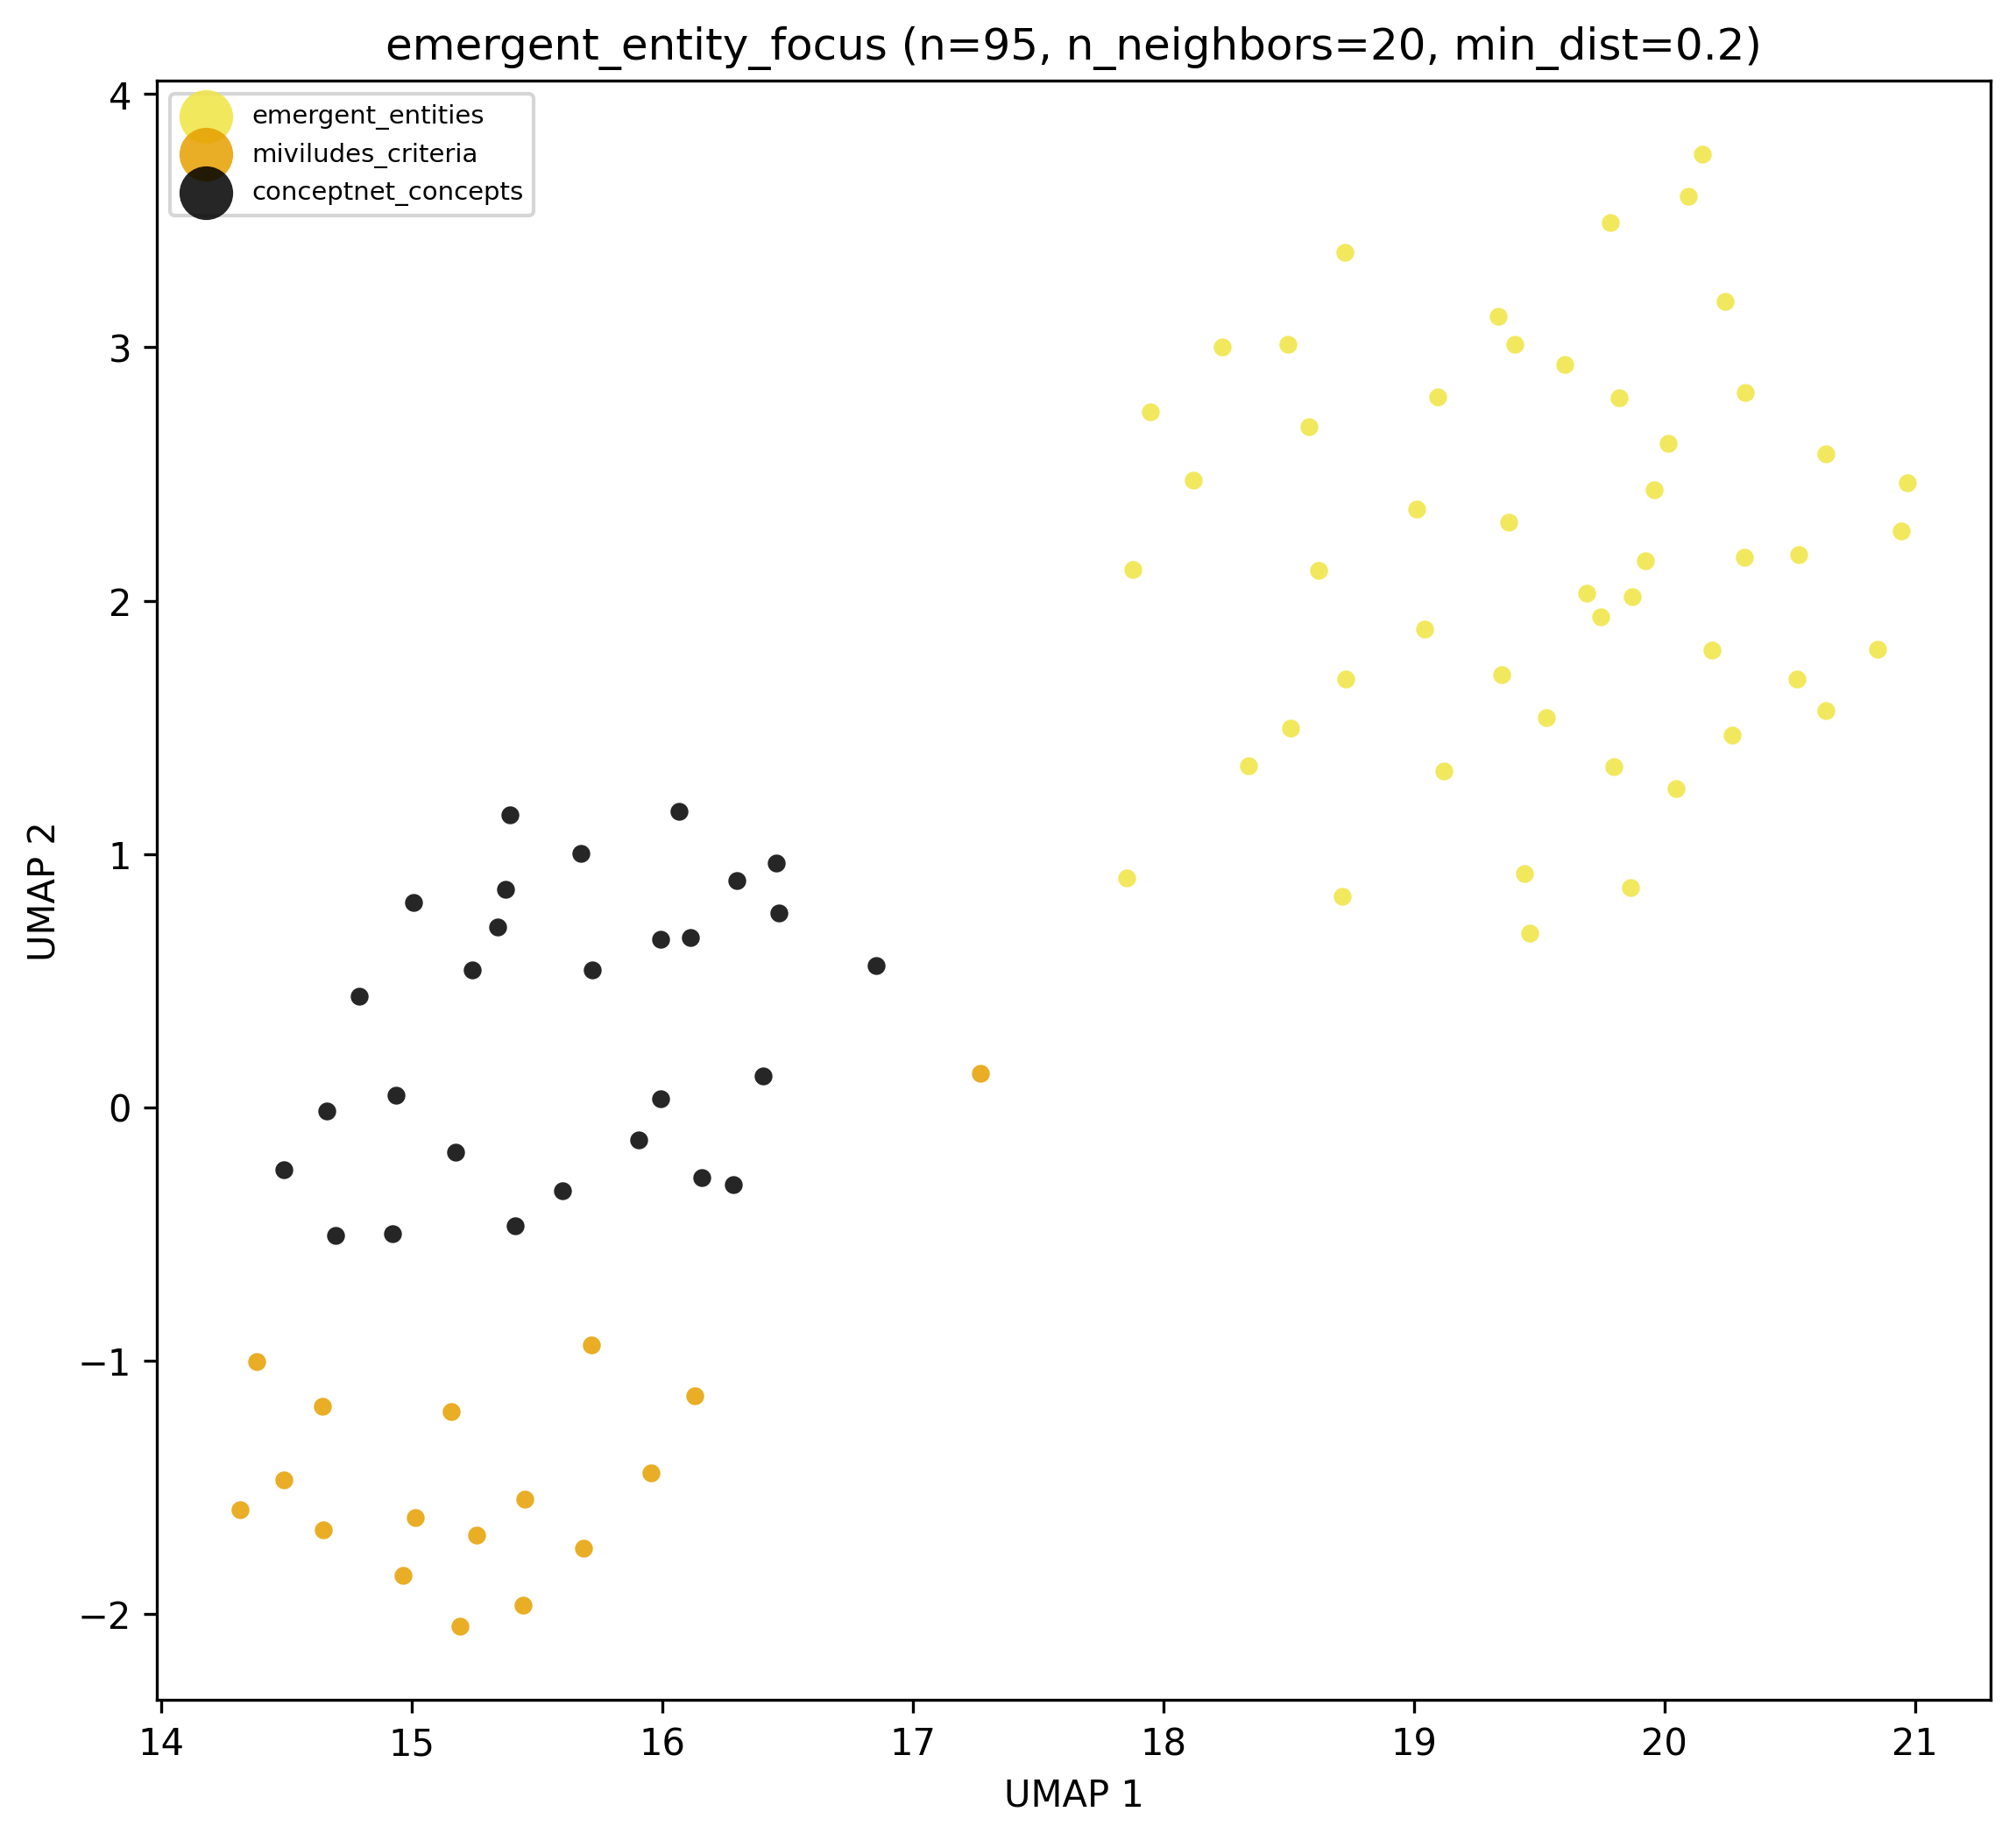
\includegraphics[width=0.8\textwidth]{figures/umap_emergent_entity_focus_by_source_dataset_n20_d0.2.png}
\caption{Focused UMAP of the top 50 emergent entities (plus neighbourhood context), coloured by source dataset -- the first version of this figure worth showing, now that the entity layer has real content.}
\end{figure}

% ============================================================
\section{Honesty notes -- what these numbers do not show}
\label{sec:honesty}
% ============================================================

\begin{itemize}[leftmargin=1.4em]
  \item \textbf{Corpus imbalance persists}: literature is 97.09\% of
  expression points; equal-$n$/equal-size corrections remain necessary
  and are used throughout.
  \item \textbf{The equal-$n$ draw is 64 points}, not v1's 204 --
  every bootstrapped CI in this document rests on a smaller sample.
  \item \textbf{The entity-layer fix is a substantial improvement, not a
  finished, hand-verified list.} Casing + per-corpus frequency + a
  corpus-author stop-list catches most noise; externally-cited classical
  theorists not among this corpus's own 57 authors are a known,
  unfixed residual (Section~\ref{sec:entities}).
  \item \textbf{French/English entity variants do not automatically
  merge.} "Scientology" (English) and "la scientologie" (French) are
  normalized and counted as separate entities unless the exact same
  string recurs -- so a genuinely shared concept can undercount as
  \texttt{shared\_all\_3} if each corpus happens to use a different-language
  form. The 3 \texttt{shared\_all\_3} entities found are a floor, not a ceiling.
  \item \textbf{MIVILUDES is still two documents}, 108 expressions.
  \item \textbf{The interview sample is a convenience sample}, 64
  expressions across 26 people.
  \item \textbf{\texttt{response\_rank} is still not usable} as a
  "first thing they thought of" signal.
  \item \textbf{One point ("Sept?") carries no propositional content}
  despite passing every automated check -- 1/11,378, negligible scale,
  real case.
  \item \textbf{Equal-size-controlled comparisons control for pool size
  only.}
  \item \textbf{2-D pictures are a reading aid, not evidence.}
  \item \textbf{Typicality/borderline scores are purely geometric}, not
  a claim about cognitive prototypicality or real-world category
  membership.
\end{itemize}

% ============================================================
\section{Possible interpretations}
\label{sec:interpretation}
% ============================================================

\begin{plainbox}[Read this box before the rest of this section]
Everything above this point is descriptive. Everything here is a
provisional \emph{reading} of that description, offered because it was
explicitly requested as a first pass -- not proof. Each is paired with a
reason it might be wrong.
\end{plainbox}

\begin{interpbox}[On what the entity fix itself shows]
The gap between 21 and 753 entities -- a 36-fold difference from a
methodology bug, not a change in the underlying corpus -- is itself
informative: it demonstrates how sensitive a "count of named things"
statistic is to exactly which extraction field it draws from, and by
extension how much scrutiny any single such count deserves before being
treated as evidence about what a corpus "really" emphasizes. One
reading: this argues for treating any single emergent-entity number in
this thesis (this run's 753 included) as provisional pending further
cross-checks, not as a finished census. \textbf{Why this might overstate
the point}: the specific bug found here (only extracting entities from
already-kept expressions) is a one-off implementation gap tied to this
particular two-field extraction schema, not evidence that the corrected
753-entity count itself is still substantially incomplete -- the fix
targeted a known, specific mechanism, not a general suspicion.
\end{interpbox}

\begin{interpbox}[On the 3 shared\_all\_3 entities]
"New Age," Jehovah's Witnesses, and the Order of the Solar Temple being
the only entities mentioned by all three corpora -- an academic
literature review, a French state agency's operational report, and 26
lay interviews -- is a narrow but suggestive overlap: two are specific,
well-known, historically prominent named groups (one linked to a mass
murder-suicide, the Solar Temple), and one is a broad, loosely-bounded
movement label. One reading: what these three very differently-motivated
sources agree is worth naming at all skews toward either extremely
notorious specific cases or extremely broad umbrella categories, with
comparatively little shared middle ground. \textbf{Why this might be
wrong}: with only 3 data points, and given the previous interpbox's
point about French/English variants not auto-merging, this could easily
be undercounting genuinely shared entities that happen to be phrased
differently per corpus (e.g., Scientology is very likely discussed by
all three under different exact strings) -- 3 is a floor, and the
pattern reading above is built on a small, possibly incomplete sample.
\end{interpbox}

\begin{interpbox}[On 55 interviews-only entities appearing for the first time]
The first v2 pass found zero interview-specific entities; this run finds
55 (Netflix, "AI cult," Blue \"Oyster Cult, Richard Branson, "Tomato
cult," and others), none overlapping literature or MIVILUDES. One
reading: lay interviewees' spontaneous associations with "cult" draw on
a genuinely different reference set than either academic literature or
state institutional framing -- pop culture, personal media consumption,
loose/metaphorical usage -- rather than simply being a smaller, noisier
version of the same discourse. \textbf{Why this might be wrong}: at
min-mentions$\geq$1 for interviews, a single interviewee's one-off
remark is enough to create an entity, so some of these 55 may be
idiosyncratic to one person rather than any kind of shared "interview
discourse" pattern -- the count says these entities are
\emph{interview-exclusive}, not that they are \emph{common} within
interviews.
\end{interpbox}

% ============================================================
\section{Using this document to write the Results chapter}
% ============================================================

Section~\ref{sec:entities} is unusually long for a "results" report
because the correction it documents is itself a methodologically
relevant fact -- how a bug in a two-field extraction schema silently
discarded most named-entity signal, and what three independent,
data-checked fixes (casing filter, a filter bug, a corpus-derived
stop-list) it took to recover it, is exactly the kind of thing a
Methods chapter should be candid about. Section~\ref{sec:interpretation}
remains a first, provisional pass, kept structurally separate from
descriptive fact throughout, offered as a starting point for argument,
not a finished answer.

\end{document}
